\documentclass[12pt]{article}

% Packages
\usepackage[margin=1in]{geometry}
\usepackage{amsmath}
\usepackage{amssymb}
\usepackage{amsthm}
\usepackage{enumitem}
\usepackage{fancyhdr}
\usepackage{tikz}
\usetikzlibrary{arrows.meta, positioning}

% Header and footer
\pagestyle{fancy}
\fancyhf{}
\lhead{CSCE 423 -- Homework 1}
\rhead{Due: February 5, 2026}
\cfoot{\thepage}

% Title information
\title{CSCE 423: Algorithms and Complexity\\Homework 1}
\author{Caleb List, Delaney Lawrence, Aiden Makovicka}
\date{Due: February 5, 2026}

\begin{document}

\maketitle

% Problem 1
\section*{Problem 1}

\subsection*{Algorithm}

For this problem we will divide our algorithm into 3 steps which involve the use of median of medians or the \texttt{SELECT} algorithm. The steps will be:

\begin{enumerate}
    \item \texttt{SELECT}$(A, j) \rightarrow a$
    \item \texttt{SELECT}$(A, k) \rightarrow b$
    \item Simple comparison loop through list to find all $x \in A$ where
    \[
        a \le x \le b.
    \]
    This would be equivalent to $j \le \text{RANK}(x) \le k$.
\end{enumerate}

\subsection*{Analyzing Time Complexity}

We have proven in class \texttt{SELECT} or median of medians is $O(n)$. Step three is a simple loop through all elements of $A$ so has a time complexity of $O(n)$. So,
\[
O(n) + O(n) + O(n)
\]
is our time complexity. Or,
\[
O(n).
\]

\subsection*{Proof of Correctness}

Given how we know \texttt{SELECT} is correct:

\begin{itemize}
    \item \texttt{SELECT}$(A, j) \rightarrow a$ is the element of rank $j$
    \item \texttt{SELECT}$(A, k) \rightarrow b$ is the element of rank $k$
\end{itemize}

If our algorithm outputs an element $x$, then $a \le x \le b$. So, there are at least $j$ elements $\le x$ and at most $k$ elements $\le x$. So,
\[
\text{RANK}(x) \in [j, k]
\]
and all output elements are correct.

If element $x$ has $\text{rank}(x) \in [j, k]$, then $x$ is between the $j^{\text{th}}$ and $k^{\text{th}}$ smallest elements. So, $a \le x \le b$ and $x$ is an output. Therefore all correct elements are output.


\vspace{1cm}

% Problem 2
\section*{Problem 2}

\subsection*{Algorithm Description}

The algorithm finds the \(i\)-th smallest element in two sorted lists using a recursive approach. At each step, it examines the elements at position \(\lfloor i/2 \rfloor\) in each list (or treats the value as infinity if a list has fewer than \(\lfloor i/2 \rfloor\) elements).

If the element from the first list is smaller than or equal to the element from the second list, then the first \(\lfloor i/2 \rfloor\) elements of the first list cannot contain the \(i\)-th smallest element overall. These elements are discarded, and a recursive call is made on the remaining portion of the first list and the entire second list, searching for the \((i - \lfloor i/2 \rfloor)\)-th smallest element. Otherwise, the first \(\lfloor i/2 \rfloor\) elements of the second list are discarded and a recursive call is made similarly.

The recursion continues until a base case is reached. If one list becomes empty, the algorithm returns the \(i\)-th element from the remaining list. If \(i = 1\), the algorithm returns the smaller of the first elements of the two lists.

\subsection*{Time Complexity}

At each recursive call, the algorithm compares the $\lfloor i/2 \rfloor$-th elements of the two sorted arrays and discards approximately $i/2$ elements from one of the arrays. Thus, the value of $i$ is reduced by about half at each step, while the work done per call is constant.

\[
T(i) = T(i/2) + O(1)
\]

Solving this recurrence gives:

\[
T(i) = O(\log i)
\]

Since $i \leq |X| + |Y|$, the overall time complexity is:

\[
T = O(\log(|X| + |Y|))
\]

\vspace{1cm}

% Problem 3
\section*{Problem 3}
To find the maximum number of shortest paths, we can use a modified BFS approach since it naturally finds the shortest path distance.

\subsection*{Initialization}

We initialize three arrays that loop through each vertex $v \in V$:
\begin{itemize}
    \item A distance array $dist[v] = \infty$ that stores the shortest distance from the source $s$.
    \item A path array $paths[v] = 0$ that stores the number of shortest paths from $s$.
    \item A Boolean array $visited[v] = \text{false}$ that stores whether or not the vertex has been visited.
\end{itemize}

Given the source $s$, we set $dist[s] = 0$ and $paths[s] = 1$. We then enqueue $s$ into a queue $Q$.

\subsection*{BFS Traversal}

While $Q$ is not empty, we dequeue a vertex $u$. For each neighboring vertex $v$ of $u$:

\begin{enumerate}
    \item If $v$ is undiscovered (i.e., $dist[v] = \infty$), we have found a shortest path to $v$. We set:
    \[
        dist[v] = dist[u] + 1
    \]
    \[
        paths[v] = paths[u]
    \]
    We then enqueue $v$ into $Q$.
    
    \item If $v$ is discovered (i.e., $dist[v] \neq \infty$) and $dist[v] = dist[u] + 1$, this represents another valid shortest path to $v$ via $u$. We update:
    \[
        paths[v] = paths[v] + paths[u]
    \]
    
    \item If $dist[v] < dist[u] + 1$, we do nothing.
\end{enumerate}

\subsection*{Finding the Maximum}

Once the queue is empty, we iterate through the $paths$ array and return the vertex with the greatest path value.

\subsection*{Time Complexity}

All vertices are enqueued and dequeued once, and each edge is only explored once. Therefore, the time complexity is $O(V + E)$.

\vspace{1cm}

% Problem 4
\section*{Problem 4}

\subsection*{Algorithm}

This problem is always asking for the 19th element we will simply loop through $A$, of size $n$, 19 times. Steps are as follows:

\begin{enumerate}
    \item Check if array length $\ge 19$
    \item Loop through array keeping track of smallest element
    \item Put smallest element at index (iteration) $\rightarrow$ first case 0
    \item Now loop from position 1 to $n-1$, finding smallest and swapping w/ position 1
    \item Keep doing this for all 19 iterations
    \item Return element $A[18]$
\end{enumerate}

We are partially sorting the array.

\subsection*{Time Complexity}

Total iterations is
\[
\sum_{i=0}^{18} (n - i - 1)
\quad \text{or} \quad
\sum_{i=1}^{19} (n - i)
= 19n - 190
\]

So,
\[
T(n) = 19n - 190 \le 19n \le cn = O(n)
\]

\subsection*{Proof of Correctness}

This algorithm is essentially the first 19 steps of selection sort. We have proved selection sort's correctness within class or prerequisites. Given this it has elements located at $A[i-1]$ where $i$ is the RANK of these elements.

Therefore,

Position $A[18]$ after our algorithm is the 19th element of $A$.

\vspace{1cm}

% Problem 5
\section*{Problem 5}

Consider the directed graph $G = (V,E)$ where
\[
V = \{s,a,b,c,d\}
\]
and
\[
E = \{(s,a), (s,b), (a,c), (a,d), (b,c), (b,d)\}.
\]

All edges have equal weight $1$. This graph is shown below.

\begin{center}
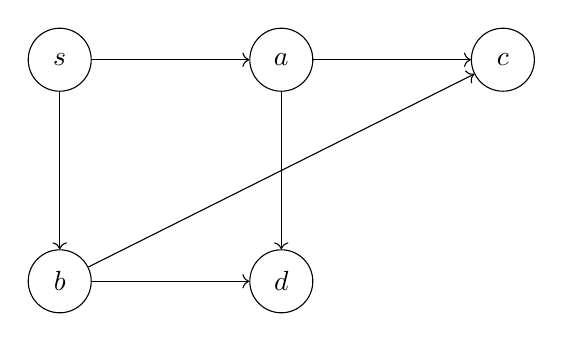
\begin{tikzpicture}[
    node distance=2cm,
    every node/.style={circle, draw, minimum size=8mm},
    every edge/.style={draw, ->}
]

\node (s) {$s$};
\node (a) [right=of s] {$a$};
\node (c) [right=of a] {$c$};

\node (b) [below=of s] {$b$};
\node (d) [right=of b] {$d$};

\draw (s) edge (a);
\draw (s) edge (b);

\draw (a) edge (c);
\draw (a) edge (d);

\draw (b) edge (c);
\draw (b) edge (d);

\end{tikzpicture}
\end{center}

\bigskip

Now define the edge set
\[
E_p = \{(s,a), (s,b), (a,c), (b,d)\}.
\]

This subgraph is shown below.

\begin{center}
\begin{tikzpicture}[
    node distance=2cm,
    every node/.style={circle, draw, minimum size=8mm},
    every edge/.style={draw, ->}
]

\node (s) {$s$};
\node (a) [right=of s] {$a$};
\node (c) [right=of a] {$c$};

\node (b) [below=of s] {$b$};
\node (d) [right=of b] {$d$};

\draw (s) edge (a);
\draw (s) edge (b);

\draw (a) edge (c);
\draw (b) edge (d);

\end{tikzpicture}
\end{center}

\bigskip

\subsection*{Requirement 1}

Each path in $(V,E_p)$ from $s$ to any vertex $v$ is a shortest path in $G$.

\medskip

The shortest path distances in $G$ are:
\begin{align*}
d(s,a) &= 1 \quad \text{via } s \rightarrow a \\
d(s,b) &= 1 \quad \text{via } s \rightarrow b \\
d(s,c) &= 2 \quad \text{via } s \rightarrow a \rightarrow c \text{ or } s \rightarrow b \rightarrow c \\
d(s,d) &= 2 \quad \text{via } s \rightarrow a \rightarrow d \text{ or } s \rightarrow b \rightarrow d
\end{align*}

In $(V,E_p)$, the paths $s \rightarrow a$ and $s \rightarrow b$ have length $1$, while the paths $s \rightarrow a \rightarrow c$ and $s \rightarrow b \rightarrow d$ have length $2$. These path lengths match the shortest path distances in $G$, so Requirement 1 is satisfied.

\bigskip

\subsection*{Requirement 2}

The edge set $E_p$ cannot be produced by a breadth-first search.

Breadth-first search uses a FIFO queue. The execution of this search will be:
\begin{enumerate}
    \item Vertex $s$ is dequeued first, and its neighbors $a$ and $b$ are enqueued.
    \item Next, either $a$ or $b$ is dequeued.
    \begin{itemize}
        \item If $a$ is dequeued first, all of its outgoing edges are discovered, namely to $c$ and $d$. Vertex $a$ becomes the parent of both, resulting in the BFS tree
        \[
        \{(s,a), (s,b), (a,c), (a,d)\}.
        \]
        \item If $b$ is dequeued first, then $b$ becomes the parent of both $c$ and $d$, resulting in the BFS tree
        \[
        \{(s,a), (s,b), (b,c), (b,d)\}.
        \]
    \end{itemize}
\end{enumerate}

In either case, BFS assigns the same parent to both $c$ and $d$. Therefore, it is impossible for $a$ to be the parent of $c$ while $b$ is the parent of $d$, as in $E_p$. Hence, $E_p$ cannot result from a BFS traversal.


\vspace{1cm}

% Problem 6
\section*{Problem 6 (Bonus)}

We can use proof by contradiction to show that the algorithm will also find the $i - 1$ smaller and $n - i$ larger elements.

We can let variable $y$ represent the $i$th smallest element returned by the algorithm. For $y$ to be the $i$th smallest, there has to be a set of $i - 1$ elements such that for all elements in the subset $a$, the element is less than $y$. There also has to be a set of exactly $n - i$ elements such that for all elements in the subset $b$, all elements are greater than $y$.

Suppose the algorithm ends early and there is an element $w$ that is not equal to $y$, and the comparison between the two elements was not determined. Without the comparison, we could change the value of $w$ to be smaller or larger than $y$ without contradicting any comparisons. Changing the value of $w$ to be greater or less than $y$ will change the rank of $y$.

This means that for the algorithm to be correct, it must have done enough comparisons to fix the rank of $y$ to be exactly $i$. This means that every element in the list has a relationship through direct comparison or the transitive property of $y$. This therefore proves that to know $y$ is the $i$th element in the list, we implicitly partition the elements into two sets, one that is less than $y$ and another greater than $y$. \qed


\end{document}


